\chapter{Introduction}
\label{chapter:one}


Modern software systems nowadays provide configuration options to modify
both functional behavior of the system, i.e. functionality of the system, and non-functional properties of the system, such as performance and memory
consumption. 
Configuration options of a software system that are relevant to users are usually referred to as
features. All the features of a system (vector of configuration options) together defines a \textit{configuration} of a software system. The features can often taken integer, decimal or string values.  One of the most important non-functional properties is performance, because it  influences the how a user interacts with the system. 
Performance can be influenced by many factors including the environment (for example, the hardware in which the software system is current executing).  A software system is required to select and set configuration options to maximize the performance of that system. For example, say we have a software system with 10 (binary) configuration options---it results in a configuration space of size $2^{10}$ or $1024$. The user of the software system, now has to find the optimal configuration for the given task (or input) in hand. 
This problem can be tackled in two different ways: (1) exhaustively measuring performance of all possible configurations---which means running 1024 benchmark runs, and (2) use domain knowledge (assuming the user has tuned similar software system before) to find the best configuration. 
However, as the number of configuration options increase, it
becomes difficult for humans to keep track of the interactions between the configuration options. This means as the configuration space grows (size of the configuration space grows exponentially) it is harder to either exhaustively measure performance for all possible configurations or find domain experts to confidently do so. Please note that the optimal configuration we are trying to find can change dramatically with different inputs (tasks) and the environment---which make domain knowledge based decision less reliable. 

This exact problem has been reported by numerous researchers from different domains.
\begin{itemize}
\item Many software systems have poorly chosen defaults [1], [2]. Hence, it is useful to seek better configurations.
\item Understanding the configuration space of software systems with large configuration spaces is challenging [3].
\item Exploring more than just a handful of configurations is usually infeasible due to long benchmarking time [4].
\end{itemize}


The problem we are trying to tackle throughout this document is: "How can be find a set of configuration options which would \underline{maximize} the performance of a system while \underline{minimizing} the cost of search". Here were would limit our scope of study to just the configurations options or features of a particular software system (and not its environment). 

\begin{figure}[!htbp]
    \centering
    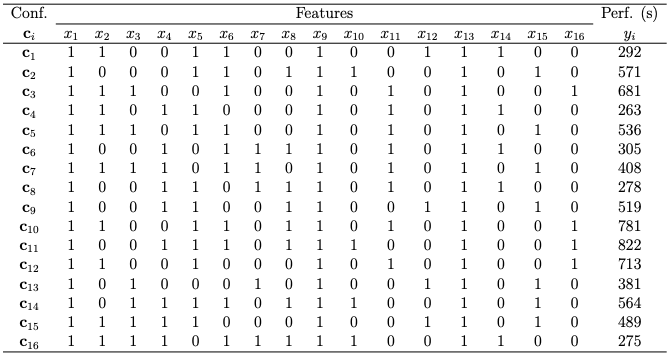
\includegraphics[width=0.8\linewidth]{Figures/table.png}
    \caption{A sample of 16 randomly-selected configurations of x264 and corresponding
performance measurements (seconds)}
    \label{fig:chap1_random_sample}
\end{figure}

\section{Motivating Example}
To motivate our work, we use the same example from a previous work~\cite{guo2013variability}, a configurable
command-line tool x264 for encoding video streams into the H.264/MPEG-4 AVC format.
In this example, we consider 16 encoder features of x264, such as encoding with multiple
reference frames and parallel encoding on multiple CPUs. The user can select
different features to encode a video. The encoding time is used to indicate the performance
of x264 in different configurations. A configuration represents a program variant with
a certain selection of features. This example with only 16 features gives rise to 1,152
configurations. Intuitively, 16 binary features should provide 216 different configurations,
however, in this work we consider only valid configurations i.e. configurations that are
allowed by the system under investigation.
In practice, often only a limited set of configurations can be measured, either by simulation
or by monitoring in the field. For example, Figure~\ref{fig:chap1_random_sample} lists a sample of 16 randomly selected
configurations and their actual performance measurements. How can we determine
the performance of other configurations based on a small random sample of measured configurations?
To formulate the above issue, we represent a feature as a binary decision variable x (please note that decision variable could be decimal as well).
If a feature is selected in a configuration, then the corresponding variable is set to 1, and
0 otherwise. Assume that there are $N$ features in total, all features of a program are
represented as a set $X = {x_1, x_2, ..., x_N}$. A configuration is an N-tuple c, assigning 1 or 0
to each variable. For example, each configuration of x264 is represented by 16-tuple, e.g.
$c_1$ = ($x_1$ = 1, $x_2$ = 1, $x_3$ = 0, $x_4$ = 0, ..., $x_{16}$ = 1). All valid configurations of a program are
denoted by $C$.
Each configuration $c$ of a program has an actual measured performance value y. Performance values are taken from publicly available dataset deployed with SPLConqueror
tool.
All performance values of all configurations $C$ form set $Y$ . Suppose that we acquire a
random sample of configurations $C_S \in C$ and their actual measured performance values
$Y_S \in Y$ , together forming sample $S$. The problem of variability-aware performance prediction
is to predict the performance of other configurations in $C \ CS$ based on the measured
sample S.
We regard all variables in X as predictors and a configuration\textquotesingle s actual performance
value y as the response. In other words, we predict a quantitative response y based on a
set of categorical predictors X, which is a typical regression problem. \textit{Due to feature
interactions, the above issue is reduced to a non-linear regression problem, where the
response depends non-linearly on one or more predictors.}




\section{Dual Axis: Quality and Cost}
\noindent\textbf{Quality}: Quality of an approach refers to the distance between the solutions returned by the techniques proposed and the ground truth. Quality can be calculated as the rank difference which is the distance between best solution (also referred to as configuration) found by (proposed) techniques to the actual best solution.

\noindent\textbf{Cost}: Cost of an approach refers to the effort required by an approach to find a good configurations. In this thesis, we use number of measurements (or benchmark runs) as an proxy to the search effort.

\begin{figure}[!htbp]
    \centering
    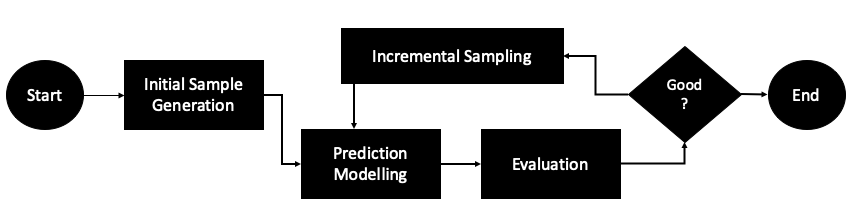
\includegraphics[width=0.8\linewidth]{Chapter-Introduction/Figures/sampling_process.png}
    \caption{ General process of performance prediction by sampling}
    \label{fig:chap1_sampling_process}
\end{figure}

\section{Prior Work}
Figure~\ref{fig:chap1_sampling_process} illustrates the general process of performance prediction by sampling. It starts with
an initial sample of measured configurations, which are used to build the prediction model. A
good initial sample significantly reduces the iterations of the entire prediction process. State-of-the-art
approaches fix the size of the initial sample to the number of features or potential feature
interactions of a system~\cite{siegmund2012predicting, guo2013variability}. However, such a strategy might not be the optimal one, as the
number of features (and their interactions) can be high and, at the same time, an acceptable prediction
accuracy might be achieved using a substantially smaller set of measured configurations.

\noindent\textbf{Observation}: Even though, the strategies proposed by earlier work in this domain exploited random sampling and CART decision trees (which are both scalable), there is repeated work. In our two axis' of evaluation, these strategies work well in the quality aspect however, does not fare well in the cost aspect. Most of the method use over 50\% of the configurations (from the configuration space), to build a reliable model. 

\section{Contributions}

\subsection{Clustering}
The prior work in this area~\cite{guo2013variability, sarkar2015cost} used a combination of random sampling and regression trees. However, random sampling completely disregards the presence of clusters in the configuration space. It has been shown in the literature~\cite{oh2017finding} that (1) most of the configuration options does not influence the performance i.e. only a few configurations options are useful, and (2) the performance curve is generally a step function. 

\begin{figure}[!htbp]
    \centering
    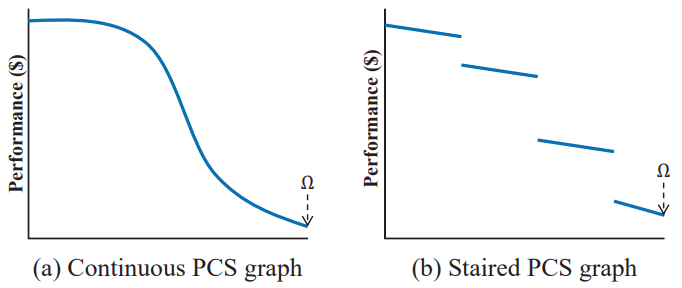
\includegraphics[width=0.8\linewidth]{Chapter-Introduction/Figures/stairs.png}
    \caption{Performance curves. (From ~\cite{oh2017finding})}
    \label{fig:chap1_stairs}
\end{figure}

To elaborate, if we sort the configurations from worst-performance to best and
plot configurations along the X-axis and performance along the
Y-axis. We expected a continuous graph
such as Figure~\ref{fig:chap1_stairs}(a), where high-valued (\$) is bad (worst performance is at the far left) and low-valued (\$) is good (best performance is at the
far right). Ω anchors the far-right point on X-axis of graphs. Interestingly, Marker et al.~\cite{marker2014understanding} discovered that performance curves often occurs (in real world) as stairs, as in Figure 3b. Stairs arise from discrete feature decisions;
some features are highly-influential in performance while others
have little or no impact. Consequently, a few critical features
influences the performance while less important feature decisions alter the performance of nearby configurations only slightly (giving a stair its width and slope).

\noindent\textbf{Intuition}: From the literature, it is evident that most of the configuration options in a (given) software system does not affect the performance of the configurations. Hence, the central insight of this work is that random sampling with no regards to this specific feature of this problem is ineffective and hence adds additional cost. 

\noindent\textbf{Proposal}: This problem can be reformulated as a clustering problem, where we try to find an unsupervised method to cluster the configuration space into meaningful clusters. Once we have this cluster (top-down bi-cluster), we can only use random sampling from each of the clusters. This way, we can reduce redundant measurements (measurements which do not provide new information).  

\subsection{Ranking}
Prior work in this area (including~\cite{nair2017faster}), tried to build accurate performance predictors, which (once trained) can be used to predict the performance of a certain configuration. This work reflects on the prior work and asks: ``\textit{Our goal is to find a good configuration~\footnote{Good is defined as the distance from the optimal configuration} but, why does the prior work transform this problem into building an accurate model?}'' Another reason for this question is the very nature of the model building process (previously described in Figure~\ref{fig:chap1_sampling_process}). We ask the question ``How does a user define \textit{Good}''? There is no way for the user to know whether a model can be build with MMRE (Mean Magnitude of Relative Error) less that 10\%. 

Considering the above mentioned questions, we drastically modify our approach to this problem. We hypothesize that to find the best performing configuration, we do not want a model which can return a predicted performance score which is as close to the actual performance score. Instead, we can build a model which preserves the relative ordering of the configurations. 

\noindent\textbf{Intuition}: The central insight of this work is that exact performance
values (e.g., the response time of a software system) are not
required to rank configurations and to identify the optimal one. To elaborate more, let us assume that we have two humans (Adam---134cm, Billy---173cm) (analogous to configurations) and our objective is to identify the tallest person (Billy). To identify the tallest person, do we need a model which accurately predicts their height in a nano-meter scale? We can easily identify Billy even if the bad model predicted Adams height as 700cm and 890cm. 

\noindent\textbf{Proposal}: 
We show that, if we (slightly) relax the question
we ask, we can build useful predictors using very small sample sets.
Specifically, instead of asking ``How long will this configuration
run?'', we ask instead ``Will this configuration run faster than that
configuration?'' or ``Which is the fastest configuration?''.


\subsection{Sequential-Model Based Sampling}
Prior work in this area primarily used two strategies.
Firstly, researchers used machine learning to model the configuration
space. The model is built sequentially, where new
configurations are sampled randomly, and the quality or
accuracy of the model is measured using a holdout set. The
size of the holdout set in some cases could be up to 20\% of
the configuration space~\cite{nair2017using} and needs to be evaluated (i.e.,
measured) before even the model is fully built. This strategy
makes these methods not suitable in a practical setting since
the generated holdout set can be (very) expensive. Secondly,
the sequential model-based techniques used in prior work
relied on Gaussian Process Models (GPM) to reflect on the
configurations explored (or evaluated) so far~\cite{zuluaga2016varepsilon}. However,
GPMs do not scale well for software systems with more than
a dozen configuration options~\cite{wang2016bayesian}.



\noindent\textbf{Intuition}: 
To reduce the cost of sampling and eliminate the need for holdout set, we use sequential Model-based Optimization (SMBO). SMBO uses the Bayesian methodology to the iterative optimizer by incorporating a prior model (built using configuration which are already measured) on the space of possible target functions, $f$. By updating this model every time time a configuration is evaluated, a SMBO routine keeps a posterior model of the target function $f$. This posterior model is the surrogate $f*$ for the function f (ground truth). Figure~\ref{fig:chap1_smbo} encapsulates the process.

\begin{figure}[!htbp]
    \centering
    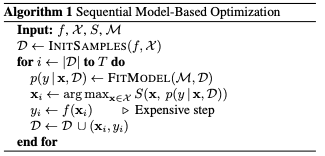
\includegraphics[width=0.8\linewidth]{Chapter-Introduction/Figures/bayesian_opt.png}
    \caption{Sequential Model-based Optimization. (From ~\url{http://tiny.cc/3hy80y})}
    \label{fig:chap1_smbo}
\end{figure}

\noindent\textbf{Proposal}:
We use the intuition present above to develop a technique called FLASH.
The key idea of FLASH is to build a performance model
that is just accurate enough for differentiating better configurations
from the rest of the configuration space. Tolerating
the inaccuracy of the model is useful to reduce the cost
(measured in terms of the number of configurations evaluated)
and the time required to find the better configuration.
To increase the scalability of methods using GPM (Gaussian Process Models)---used widely in the machine learning domain, FLASH
replaces the GPMs with a fast and scalable decision tree learner.




This dissertation is organized as follows.
Chapter~\ref{chapter:background} presents the background and related work.
Next, Chapter~\ref{chapter:WHAT} describes the design and implementation
of \emph{WHAT}, an approach to use lower dimensions to sample configurations to build performance models to achieve accurate and robust performance prediction.
Chapter~\ref{chapter:rank} proposes using ranking models instead of regression models to save cost while finding good configurations.
In Chapter~\ref{chapter:flash}, we design and implement FLASH
, an efficient and  effective solution to software configuration problem.
Finally, Chapter~\ref{chapter:conclusion} concludes our discussion of software configuration tuning and describes its future directions.
